\documentclass[border=12pt]{standalone}
\def\pgfsysdriver{pgfsys-dvisvgm.def}
\usepackage[dvisvgm]{xcolor}
\usepackage{xeCJK}
\setCJKmainfont{HaranoAjiGothic-Regular.otf}[BoldFont=HaranoAjiGothic-Bold.otf]
\setCJKsansfont{HaranoAjiGothic-Regular.otf}[BoldFont=HaranoAjiGothic-Bold.otf]
\usepackage{amsmath,amssymb,tikz,lmodern}
\usetikzlibrary{arrows.meta,positioning,calc,fit,backgrounds}
\renewcommand{\familydefault}{\sfdefault}
\definecolor{ink}{HTML}{25322F}
\definecolor{green}{HTML}{246657}
\definecolor{tint}{HTML}{EEF4F0}
\definecolor{soft}{HTML}{C6D2CC}
\definecolor{muted}{HTML}{52615B}
\newif\ifJapanese
\newcommand{\Tx}[2]{\ifJapanese #1\else #2\fi}
\newcommand{\Eff}{\overline{\operatorname{Eff}}}
\newcommand{\heading}[3]{{\color{green}\bfseries #1\quad\Tx{#2}{#3}}\\[5pt]}
% A white rectangle makes the complete citation label clickable, including spaces.
\newcommand{\refurl}[2]{\special{dvisvgm:raw <a xlink:href="#1" target="_blank" rel="noopener noreferrer">}{\setlength{\fboxsep}{0pt}\colorbox{white}{\color{green}\underline{\strut #2}}}\special{dvisvgm:raw </a>}}
\tikzset{
 card/.style={draw=soft,fill=white,rounded corners=2pt,align=left,text=ink,font=\fontsize{10.5}{14}\selectfont,inner xsep=12pt,inner ysep=10pt,text width=14.4cm},
 half/.style={card,text width=6.45cm,minimum height=2.05cm},
 result/.style={card,draw=green,fill=tint,line width=.9pt},
 reason/.style={align=left,text=muted,font=\fontsize{9}{12}\selectfont,inner sep=0pt,text width=12.7cm},
 branchreason/.style={reason,text width=5.95cm},
 edge/.style={-{Stealth[length=2.4mm]},draw=green,line width=1pt},
 wire/.style={draw=green,line width=1pt},
}
% Keep the arrow in a dedicated left gutter; explanations never cover it.
\newcommand{\flow}[3]{
 \coordinate (#2-from) at ($(#1.south)+(-6.9,0)$);
 \coordinate (#2-to) at ($(#2.north)+(-6.9,0)$);
 \draw[edge] (#2-from)--(#2-to);
 \node[reason,anchor=west] (#2-reason) at ($(#2-from)!.5!(#2-to)+(.55,0)$) {#3};
}

\newcommand{\Cite}[2]{\refurl{#1}{#2}}

\Japanesetrue
\begin{document}
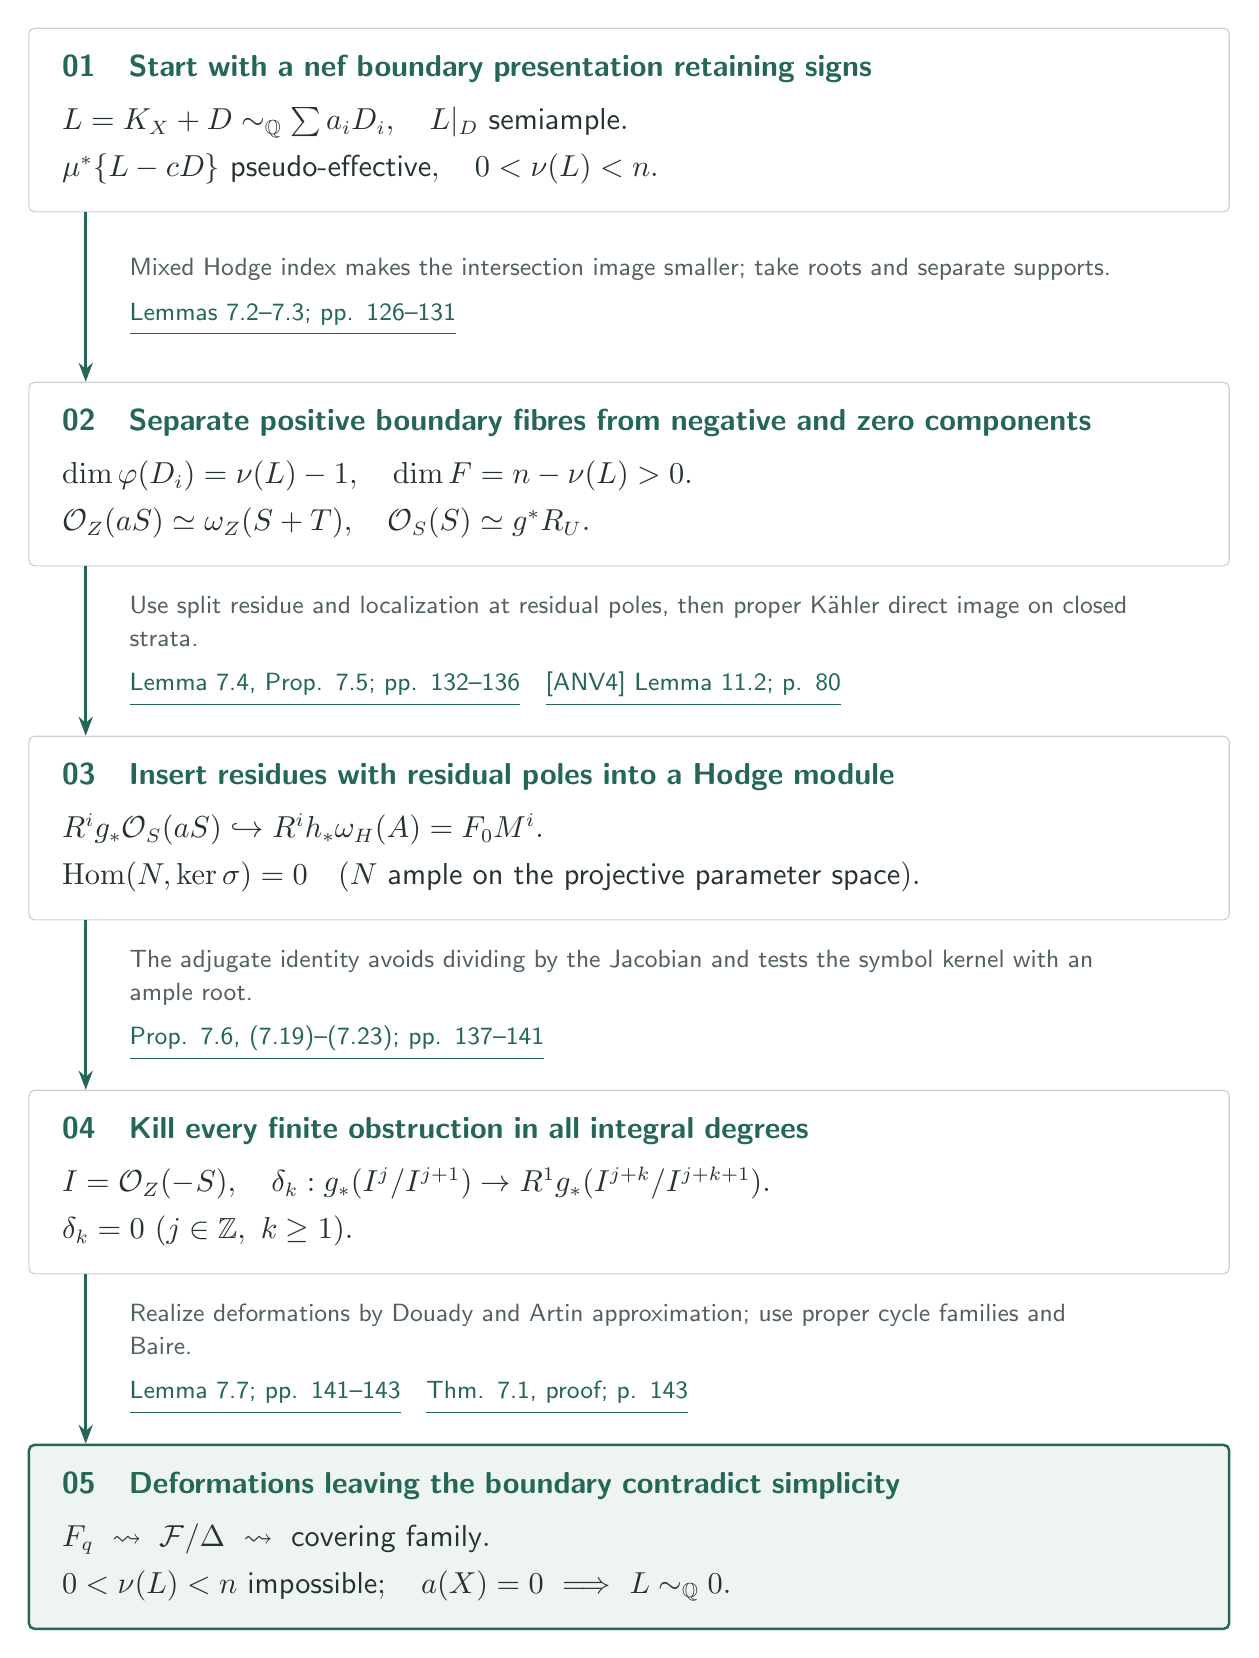
\begin{tikzpicture}
\node[card] (n0) {\heading{01}{符号を保ったnefな境界表示から始める}{Start with a nef boundary presentation retaining signs}$L=K_X+D\sim_{\mathbb Q}\sum a_iD_i,\quad L|_D\text{ semiample}.$\\[3pt] $\mu^*\{L-cD\}\text{ pseudo-effective},\quad 0<\nu(L)<n.$};
\node[card,below=2.15cm of n0] (n1) {\heading{02}{正係数の成分のファイバーを負・零成分から分離}{Separate positive boundary fibres from negative and zero components}$\dim\varphi(D_i)=\nu(L)-1,\quad \dim F=n-\nu(L)>0.$\\[3pt] $\mathcal O_Z(aS)\simeq\omega_Z(S+T),\quad \mathcal O_S(S)\simeq g^*R_U.$};
\flow{n0}{n1}{\Tx{混合Hodge indexで交わりの像を小さくし、根と分離の操作を行う。}{Mixed Hodge index makes the intersection image smaller; take roots and separate supports.}\\[4pt]\Cite{https://github.com/openai/math/blob/adc7f1241b42e322a6451854ab7e4b4c146bf78a/preprints/Log-abundance-for-compact-Kahler-spaces-under-logarithmic-Iitaka-subadditivity-October-4-2026/main.pdf}{Lemmas 7.2--7.3; pp. 126--131}}
\node[card,below=2.15cm of n1] (n2) {\heading{03}{残余極を持つ留数をHodge moduleへ入れる}{Insert residues with residual poles into a Hodge module}$R^ig_*\mathcal O_S(aS)\hookrightarrow R^ih_*\omega_H(A)=F_0M^i.$\\[3pt] $\operatorname{Hom}(N,\ker\sigma)=0\quad(N\Tx{\text{ は射影パラメータ空間上でample}}{\text{ ample on the projective parameter space}}).$};
\flow{n1}{n2}{\Tx{分裂留数と残余極の局所化。閉stratumのproper Kähler direct imageを使う。}{Use split residue and localization at residual poles, then proper Kähler direct image on closed strata.}\\[4pt]\Cite{https://github.com/openai/math/blob/adc7f1241b42e322a6451854ab7e4b4c146bf78a/preprints/Log-abundance-for-compact-Kahler-spaces-under-logarithmic-Iitaka-subadditivity-October-4-2026/main.pdf}{Lemma 7.4, Prop. 7.5; pp. 132--136}\quad \Cite{https://github.com/openai/math/blob/adc7f1241b42e322a6451854ab7e4b4c146bf78a/preprints/Abundance-after-nonvanishing-for-compact-Kahler-fourfolds-September-27-2026/paper.pdf}{[ANV4] Lemma 11.2; p. 80}}
\node[card,below=2.15cm of n2] (n3) {\heading{04}{全整数次数の全有限障害を消す}{Kill every finite obstruction in all integral degrees}$I=\mathcal O_Z(-S),\quad\delta_k:g_*(I^j/I^{j+1})\to R^1g_*(I^{j+k}/I^{j+k+1}).$\\[3pt] $\delta_k=0\ (j\in\mathbb Z,\ k\ge1).$};
\flow{n2}{n3}{\Tx{adjugate恒等式でJacobianを割らず、ampleな根からsymbol kernelへ送る。}{The adjugate identity avoids dividing by the Jacobian and tests the symbol kernel with an ample root.}\\[4pt]\Cite{https://github.com/openai/math/blob/adc7f1241b42e322a6451854ab7e4b4c146bf78a/preprints/Log-abundance-for-compact-Kahler-spaces-under-logarithmic-Iitaka-subadditivity-October-4-2026/main.pdf}{Prop. 7.6, (7.19)--(7.23); pp. 137--141}}
\node[result,below=2.15cm of n3] (n4) {\heading{05}{境界を離れる変形がsimplicityに矛盾する}{Deformations leaving the boundary contradict simplicity}$F_q\ \leadsto\ \mathcal F/\Delta\ \leadsto\ \Tx{\text{被覆族}}{\text{covering family}}.$\\[3pt] $0<\nu(L)<n\Tx{\text{ は不可能}}{\text{ impossible}};\quad a(X)=0\ \Longrightarrow\ L\sim_{\mathbb Q}0.$};
\flow{n3}{n4}{\Tx{Douady・Artin近似で変形を実現し、properなcycle族とBaireで被覆する。}{Realize deformations by Douady and Artin approximation; use proper cycle families and Baire.}\\[4pt]\Cite{https://github.com/openai/math/blob/adc7f1241b42e322a6451854ab7e4b4c146bf78a/preprints/Log-abundance-for-compact-Kahler-spaces-under-logarithmic-Iitaka-subadditivity-October-4-2026/main.pdf}{Lemma 7.7; pp. 141--143}\quad \Cite{https://github.com/openai/math/blob/adc7f1241b42e322a6451854ab7e4b4c146bf78a/preprints/Log-abundance-for-compact-Kahler-spaces-under-logarithmic-Iitaka-subadditivity-October-4-2026/main.pdf}{Thm. 7.1, proof; p. 143}}
\end{tikzpicture}

\end{document}
